\chapter{Preleminaries}
\section{Example}
The same example will be used on many places throughout this report. By explaining the example in detail here, the explanations that use it should be clearer to the reader.

Imagine a Bank that manages different bank accounts which can be identified by their name. Customers can deposit and withdraw money from their accounts by using the ATMs. The customers interact with the ATM through some kind of user interface. This user interface will be implemented in different ways (textual or graphical), depending on our use case (\figref{fig:example_class_diagram}). All operations on the bank account will be dispatched from the ATM to the bank. 

To make the example more interesting, we will some times assume that BANK accesses the network, file system and a database. This will make capture and replay of the system more difficult. %TODO: wahrscheinlich sollten wir das ins Klassen-diagramm nehmen?

 \begin{figure}[ht]
   \centering
   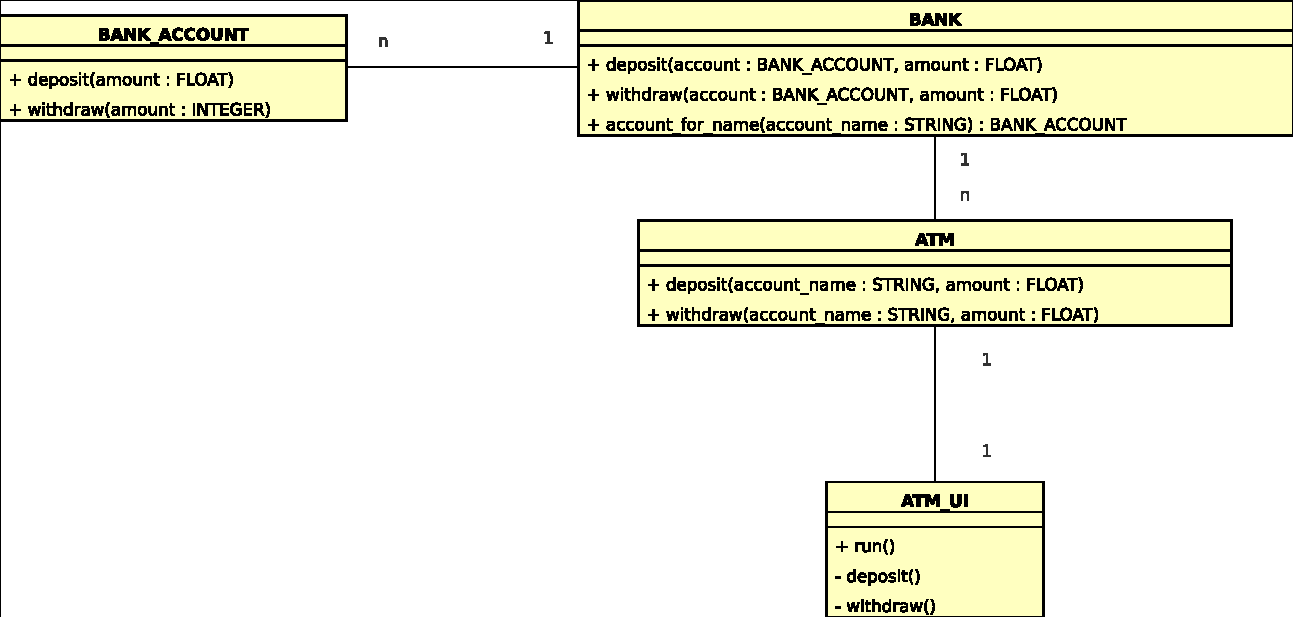
\includegraphics[width=1\textwidth]{illustrations/example_class_diagram}
   \caption{Class Diagram of the Example}
   \label{fig:example_withdraw_sequence}
 %\includegraphics{illustrations/capture_and_replay_generic_structure}
\end{figure}

One use case is money withdrawal by a customer via the ATM. The customer launches the withdrawal operation on the ATM\_UI. The request is passed through the ATM to the BANK which then withdraws the money from the Account. The sequence diagram (\figref{fig:example_withdraw_sequence}) should clarify how the classes interact with each other.

\begin{figure}[ht]
   \centering
   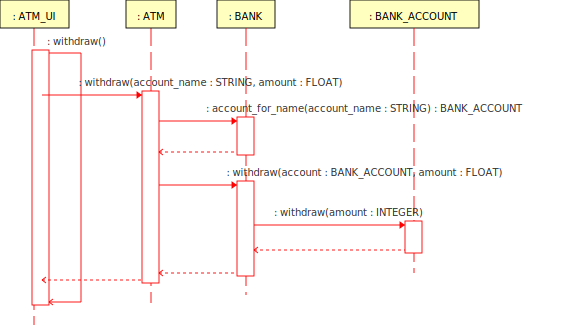
\includegraphics[width=1\textwidth]{illustrations/example_withdrawal}
   \caption{Withdrawal Operation Invoked by the User}
   \label{fig:example_class_diagram}
 %\includegraphics{illustrations/capture_and_replay_generic_structure}
\end{figure}

\section{Selective Capture and Replay}
After giving a short overview about the different capture and replay techniques, our choice will be described here in detail. This chapter summarizes papers from Joshi and Orso about the Java implementation of Selective Capture and Replay (SCARPE) \cite{orso05may, orso06}.

\subsection{Technique and Terminology}
\begin{figure}[ht]
  \centering
  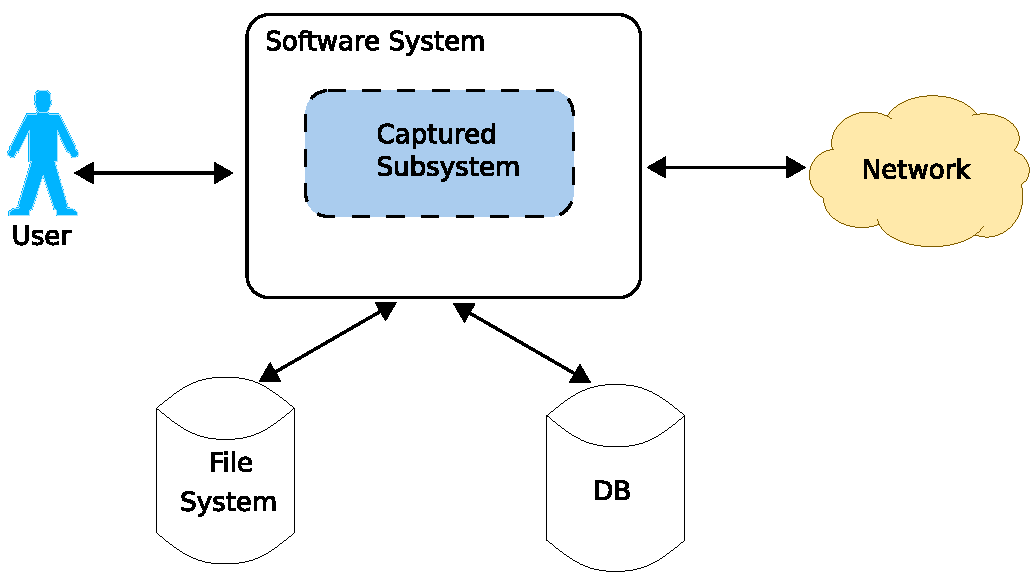
\includegraphics[width=1\textwidth]{illustrations/scr_overall_schema}
  \caption{System Layout of the Example Application (derived from \cite{orso05may})}
  \label{fig:scr_overall_schema}
%\includegraphics{illustrations/capture_and_replay_generic_structure}
\end{figure}
This technique lets the user choose the subset (\emph{captured subsystem}) of the program that should be captured and replayed (\figref{fig:scr_overall_schema}). The technique then only captures the execution data of that subsystem, ignoring the other parts of the system. The relevant interactions between the captured subsystem and the outside world is captured in terms of events; those events are read during the replay phase in order to replay the corresponding interactions. Only a part of the information that traverses the border between the captured system and the rest of the system is captured. This is significant improvement over other existing techniques, especially when big datastructures are passed over the border, but only a part of those datastructures is actually accessed.

\begin{description}
	\item [The observed set] is the subsystem that was selected for capture and replay.
	\item [The observed classes] are the classes in the observed set. Observed code is defined analogous.
	\item [Observed methods and fields] are the fields and methods of the observed classes.
\end{description}
\emph{Unobserved set},  \emph{unobserved classes}, \emph{unobserved code}, \emph{unobserved methods} and \emph{unobserved fields} are the analogous terms for the part of the system that was not selected for capture and replay.
\begin{description}
%	\item [External code]  Nur definieren, wenn es auch gebraucht wird.
	\item [Unmodifiable classes] are the classes whose code can not be modified (e.g. some system classes such as \texttt{java.lang.Class}) due to constraints from the Java Virtual Machines
	\item [Modifiable classes] are all classes except the \emph{unmodifiable classes}
\end{description}

The technique is divided in two main phases: capture and replay. \figref{fig:scr_capture_replay_phase} illustrates the structure of of these two phases in selective capture and replay.
\begin{figure}[ht]
  \centering
  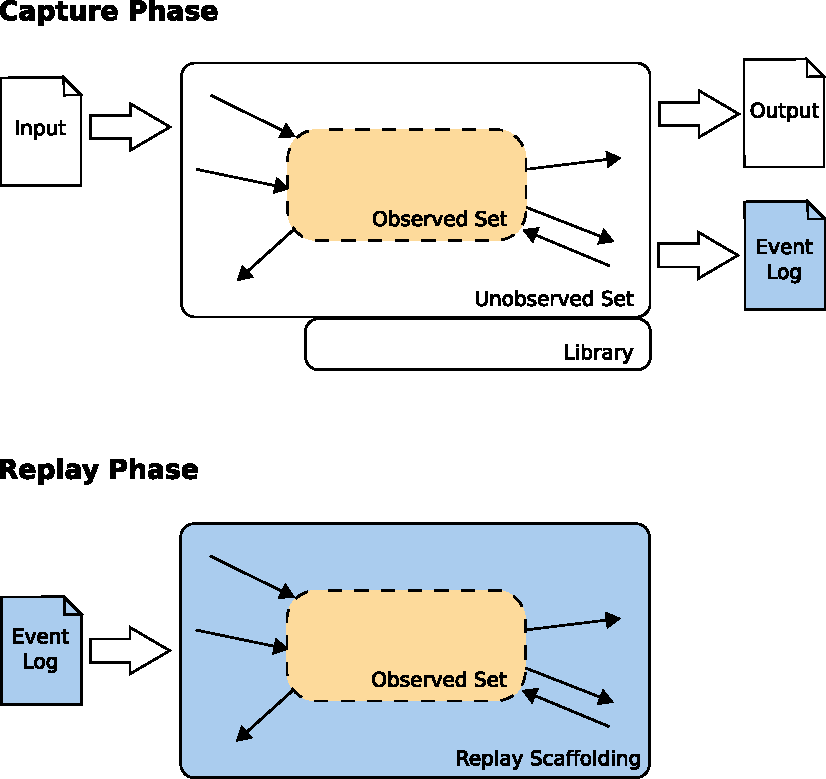
\includegraphics[width=0.8\textwidth]{illustrations/scr_capture_replay_phase}
  \caption{Capture and Replay Phase in Selective Capture and Replay}
  \label{fig:scr_capture_replay_phase}
%\includegraphics{illustrations/capture_and_replay_generic_structure}
\end{figure}
The \emph {capture phase} takes place when the application is run for recording. Before the application starts, the boundaries of the observed set are identified and the application is instrumented in order to be able to capture interactions between the observed set and the rest of the system. While the application runs, the instrumentation generates the events for these interactions and writes them to the \emph{event log}.

In the \emph{replay phase}, the technique generates the \emph{replay scaffolding}. The replay scaffolding uses the event log to replay the events on the observed set. Replaying consists both of performing actions on the observed set (e.g. invocation of a method of the observed set) and consuming actions of the observed set (e.g. receiving a method invocation originally targeted to the unobserved set). Thus the replay scaffolding acts both as a driver and stub.

\subsection{Capture Phase}
%Capture Phase
\subsubsection{Capturing Partial Information}
The technique for capturing only partial information instead of the whole data that flows into unobserved set, selective capture and replay needs an \emph{object ID}. The object ID uniquely identifies a class instance. SCARPE introduces the object ID into the program by adding an additional field to all modifiable classes. It further instruments the creation constructors of these classes so that the unique object ID is aquired from a global counter. For unmodifiable classes however, a reference map is needed to store the object ID of its instances. The object ID for instances of unmodifiable classes is acquired when it is looked up the first time. The reference map uses weak refences so that the referenced objects can be collected by the garbage collector to avoid memory leaks


%- object ID (modifiable & unmodifiable classes)
%- partial Information (different explanation than in the paper)
%- events and instrumentation (interactions observed - external code)
% -- Calls
\subsection{Replay Phase}
%Replay phase
%- Object creation
%- Events replaying